The NUHM2 interpretation in the strongly produced SUSY particles search is presented in the paper ``Searching for supersymmetry in final states with two same-sign or three leptons and jets using 36~{\ifb} of $\sqrt{s} = 13$~{\TeV} $pp$ collision data with the ATLAS detector''~\cite{Aaboud:2017dmy}.
This chapter is a complement to the NUHM2 interpretation for the same-sign or three leptons and jets search.

%%%
%%%
%%%

\section{Monte Carlo event samples and data set}
\label{app:ss3l_MC_samples}
The NUHM2 model involves gluino pair production where gluinos decay into $\ttbar \widetilde{\chi}^{0}_{1}$ and $t\bar{b} \widetilde{\chi}^{\pm}_{1}$ as shown in Fig.~\ref{fig:app_ss3l_feynman_diagram}.

\begin{figure}[htbp]
    \begin{subfigure}[b]{0.48\textwidth}
        \begin{center}
            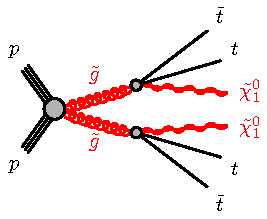
\includegraphics[scale=1.0]{gogo-ttttN1N1.pdf}
            \caption{$\widetilde{g} \to \ttbar \widetilde{\chi}^{0}_{1}$}
        \end{center}
    \end{subfigure}
    \begin{subfigure}[b]{0.48\textwidth}
        \begin{center}
            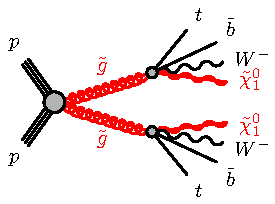
\includegraphics[scale=1.0]{gogo-ttWWbbN1N1.pdf}
            \caption{$\widetilde{g} \to t\bar{b} \widetilde{\chi}^{\pm}_{1} \to t\bar{b} W^{\pm} \widetilde{\chi}^{0}_{1}$}
        \end{center}
    \end{subfigure}
    \caption{The Feynman diagrams for the NUHM2 SUSY signal process.}
    \label{fig:app_ss3l_feynman_diagram}
\end{figure}

The Monte Carlo (MC) samples are produced to model the SUSY signals and to estimate the SM background.
A fast simulation (AFII\footnote{AFII stands for ATLAS Fast Monte Carlo II.}) based on {\GEANT}4~\cite{Agostinelli:2002hh} simulation package is used to generate the NUHM2 signal samples.
An ATLAS detector full simulation (FullSim) simulating the detailed properties of the ATLAS detector is used to produce the SM background.
The simulated MC events are re-weighted to the observed pileup conditions in the data.
Table~\ref{tab:app_ss3l_MC_samples} shows the event generator, parton shower, cross-section normalization, PDF set~\cite{Martin:2009iq}, and the set of tuned parameters for modeling for all samples.
Except those produced by the {\SHERPA}, the \textsc{EvtGEN}\xspace v1.2.0 package~\cite{Lange:2001uf} is used to model the properties of bottom and charm hadron decays for all MC samples.

\begin{table}[htbp]
    %\begin{center}
    \resizebox{\textwidth}{!}{% <------ Don't forget this %
        \begin{tabular}{ccccccc}
            \hline
            \hline
            Signal/Background                                      & Physics process                   & Event generator                  & Parton shower     & Cross-section normalization & PDF set    & Set of tuned parameters\\
            \hline
            \hline
            Signal                                                 & NUHM2                             & MG5\_{\scriptsize A}MC@NLO 2.2.3 & {\PYTHIA} 8.186   & NLO+NLL                     & NNPDF2.3LO & A14\\
            % \multirow{3}{*}{Signal}                                & RPC                               & MG5\_{\scriptsize A}MC@NLO 2.2.3 & {\PYTHIA} 8.186   & NLO+NLL                     & NNPDF2.3LO & A14\\
            %                                                        & RPV (except Figure~\ref{})        & MG5\_{\scriptsize A}MC@NLO 2.2.3 & {\PYTHIA} 8.210   & or                          & NNPDF2.3LO & A14\\
            %                                                        & RPV (Figure~\ref{})               & {\HERWIGpp} 2.7.1                & {\HERWIGpp} 2.7.1 & NLO-Prospino2               & CTEQ6L1    & UEEE5\\
            \hline
            \multirow{3}{*}{\shortstack{$t\bar{t}+X$\\background}} & $t\bar{t}W, t\bar{t}Z/\gamma^{*}$ & MG5\_{\scriptsize A}MC@NLO 2.2.2 & {\PYTHIA} 8.186   & NLO                         & NNPDF2.3LO & A14\\
                                                                   & $t\bar{t}H$                       & MG5\_{\scriptsize A}MC@NLO 2.3.2 & {\PYTHIA} 8.186   & NLO                         & NNPDF2.3LO & A14\\
                                                                   & 4$t$                              & MG5\_{\scriptsize A}MC@NLO 2.2.2 & {\PYTHIA} 8.186   & NLO                         & NNPDF2.3LO & A14\\
            \hline
            \multirow{2}{*}{\shortstack{Diboson\\background}}      & $ZZ, WZ$                          & {\SHERPA} 2.2.1                  & {\SHERPA} 2.2.1   & NLO                         & NNPDF2.3LO & {\SHERPA} default\\
                                                                   & Other (inc. $W^{\pm}W^{\pm}$)     & {\SHERPA} 2.1.1                  & {\SHERPA} 2.1.1   & NLO                         & CT10       & {\SHERPA} default\\
            \hline
            \multirow{4}{*}{\shortstack{Rare\\background}}         & $t\bar{t}WW, t\bar{t}WZ$          & MG5\_{\scriptsize A}MC@NLO 2.2.2 & {\PYTHIA} 8.186   & NLO                         & NNPDF2.3LO & A14\\
                                                                   & $tZ, tWZ, tt\bar{t}$              & MG5\_{\scriptsize A}MC@NLO 2.2.2 & {\PYTHIA} 8.186   & LO                          & NNPDF2.3LO & A14\\
                                                                   & $WH, ZH$                          & MG5\_{\scriptsize A}MC@NLO 2.2.2 & {\PYTHIA} 8.186   & NLO                         & NNPDF2.3LO & A14\\
                                                                   & Triboson                          & {\SHERPA} 2.1.1                  & {\SHERPA} 2.1.1   & NLO                         & CT10       & {\SHERPA} default\\
            \hline
            \hline
        \end{tabular}
    }
    %\end{center}
    \caption{The simulated NUHM2 SUSY signal and SM background MC samples.
    The event generator, parton shower, cross-section normalization, PDF set, and the set of tuned parameters for each samples are shown.
    The $\ttbar WW$, $\ttbar WZ$, $tZ$, $tWZ$, $t \ttbar$, $WH$, $ZH$ and triboson background samples are labeled in the ``rare'' because they contribute a very small amount to the signal region.}
    \label{tab:app_ss3l_MC_samples}
\end{table}%

The data samples are required to satisfy the following good runs list (GRLs) as recommended by the ATLAS collaboration:

\begin{itemize}
    \item \texttt{data15\_13TeV.periodAllYear\_DetStatus-v79-repro20-02\_\\DQDefects-00-02-02\_PHYS\_StandardGRL\_All\_Good\_25ns.xml}
    \item \texttt{data16\_13TeV.periodAllYear\_DetStatus-v83-pro20-15\_\\DQDefects-00-02-04\_PHYS\_StandardGRL\_All\_Good\_25ns.xml}
\end{itemize}

The integrated luminosities corresponding to these datasets are respectively 3.21~{\ifb} for 2015 and 32.86~{\ifb} for 2016.
The combined luminosity uncertainty for 2015 and 2016 is 3.2\%.

%%%
%%%
%%%

\section{Event reconstruction and signal region selection}
\label{app:ss3l_event_reconstruction_and_SR_selection}
Events are selected using the trigger strategy shown in Table~\ref{tab:app_ss3l_trigger_strategy}.
The definition of objects used in this analysis are based on the recommendations by Combined Performance groups and are summarized in Table~\ref{tab:app_ss3l_object_definitions}.

\begin{table}[htbp]
    %\begin{center}
    \resizebox{\textwidth}{!}{% <------ Don't forget this %
        \begin{tabular}{lll}
        \hline
        \hline
        Year                  & \met requirement    & triggers\\
        \hline
        \multirow{2}{*}{2015} & $\met < 250$~{\GeV} & \texttt{HLT\_2e12\_lhloose\_L12EM10VH} $\cup$ \texttt{HLT\_e17\_lhloose\_mu14} $\cup$ \texttt{HLT\_mu18\_mu8noL1}\\
                              & $\met > 250$~{\GeV} & \texttt{HLT\_2e12\_lhloose\_L12EM10VH} $\cup$ \texttt{HLT\_e17\_lhloose\_mu14} $\cup$ \texttt{HLT\_mu18\_mu8noL1} $\cup$ \texttt{HLT\_xe70}\\
        \hline
        \multirow{2}{*}{2016} & $\met < 250$~{\GeV} & \texttt{HLT\_2e17\_lhvloose\_nod0} $\cup$ \texttt{HLT\_e17\_lhloose\_nod0\_mu14} $\cup$ \texttt{HLT\_mu22\_mu8noL1}\\
                              & $\met > 250$~{\GeV} & \texttt{HLT\_2e17\_lhvloose\_nod0} $\cup$ \texttt{HLT\_e17\_lhloose\_nod0\_mu14} $\cup$ \texttt{HLT\_mu22\_mu8noL1} $\cup$ \texttt{HLT\_xe100\_mht\_L1XE50} $\cup$ \texttt{HLT\_xe110\_mht\_L1XE50}\\
        \hline
        \hline
        \end{tabular}
    }
    %\end{center}
    \caption{The trigger strategy used in the same-sign or three leptons and jets analysis.}
    \label{tab:app_ss3l_trigger_strategy}
\end{table}%

\begin{table}[htb]
    \begin{center}
        {\scriptsize
            \begin{tabular}{lll}
                \hline
                \hline
                Property                   & Preselected object                                                          & Signal object\\
                \hline
                \textbf{Electrons}         &                                                                             &\\
                \multirow{2}{*}{Kinematic} & $\pt > 10$~{\GeV},                                                          & $\pt > 10$~{\GeV},\\
                                           & $|\eta_\mathrm{clus}| < 2.47$, exclude $1.37 < |\eta_\mathrm{clus}| < 1.52$ & $|\eta_\mathrm{track}| < 2$\\
                Identification             & \texttt{LooseAndBLayerLLH}                                                  & \texttt{MediumLLH}\\
                \multirow{2}{*}{Isolation} & \multirow{2}{*}{-}                                                          & $\pt^\mathrm{varcone\ 0.2}/\pt < 0.06$\\
                                           &                                                                             & $E_\mathrm{T}^\mathrm{topocone\ 0.2}/\pt < 0.06$\\
                Impact parameter           & $|d_{0}/\sigma(d_{0})| < 5$                                                 & $|d_{0}/\sigma(d_{0})| < 5$, $|z_{0} \sin\theta| < 0.5$~mm\\
                \hline
                \textbf{Muons}             &                                                                             &\\
                Kinematic                  & $\pt > 10$~{\GeV}, $|\eta| < 2.5$                                           & $\pt > 10$~{\GeV}, $|\eta| < 2.5$\\
                Identification             & \texttt{Medium}                                                             & \texttt{Medium}\\
                Isolation                  & -                                                                           & $\pt^\mathrm{varcone\ 0.3}/\pt < 0.06$\\
                Impact parameter           & -                                                                           & $|d_{0}/\sigma(d_{0})| < 3$, $|z_{0} \sin\theta| < 0.5$~mm\\
                \hline
                \textbf{Jets}& &\\
                Kinematic                  & \multicolumn{2}{c}{$\pt > 20$~{\GeV}, $|\eta| < 2.8$}\\
                Clustering                 & \multicolumn{2}{c}{Anti-$k_{t}$ $R = 0.4$ \texttt{EMTopo}}\\
                Pileup mitigation          & \multicolumn{2}{c}{reject $\pt < 60$~{\GeV} $\cap$ $|\eta| < 2.4$ $\cap$ JVT $< 0.59$} after overlap removal\\
                $b$-tagging                & \multicolumn{2}{c}{$\pt > 20$~{\GeV}, $|\eta| < 2.5$, \texttt{MV2c10} $> 0.8244$ (70\% efficiency)}\\
                \hline
                \hline
            \end{tabular}
        }
    \end{center}
    \caption{Summary of object definitions used in the same-sign or three leptons and jets analysis.}
    \label{tab:app_ss3l_object_definitions}
\end{table}%

The objects are divided into two categories: preselected and signal objects where signal objects are a subset of preselected objects. 
Unless otherwise stated, the recommendations implemented in SUSYTools-00-08-58 and AnalysisBase 2.4.29 are used for all the objects.
The overlaps between the different objects are applied after the object identification depending on the distance $\Delta R \equiv \sqrt{(\Delta y)^{2} + (\Delta \phi)^{2}}$.
For the electron case, the jet is discarded if the $\Delta R(e, \mathrm{jet}) < 0.2$ unless the jet is a $b$-tagged jet, in which case the electron is removed.
For the muon case, if the jet has less than three associated tracks, then the muon is retained and the jet is discarded.
The remaining lepton is removed if the lepton is in a cone $\Delta R = \mathrm{min}(0.4, 0.1 + 9.6$~{\GeV}$/\pt(\ell))$ of a jet.
Events are selected if there are at least two signal leptons with $\pt > 20$~{\GeV} and two signal leptons must have the same electric charge.
Events are removed if they contain any jet not satisfying the jet requirement listed in the Table~\ref{tab:app_ss3l_object_definitions}.
The signal region is defined in Table~\ref{tab:app_ss3l_SR} to maximize the sensitivity of the NUHM2 model.
The $m_\mathrm{eff}$ in the Table~\ref{tab:app_ss3l_SR} is the scalar sum of the signal leptons \pt, jets \pt and the \met.

\begin{table}[htbp]
    \begin{center}
        {\scriptsize
            \begin{tabular}{lllllll}
                \hline
                \hline
                Signal Region & $N^\mathrm{signal}_\mathrm{lepton}$ & $N_{b\mathrm{-jets}}$ & $N_\mathrm{jets}$ & $\pt^\mathrm{jet}$~[{\GeV}] & $m_\mathrm{eff}$~[{\GeV}] & $\met/m_\mathrm{eff}$\\
                \hline
                NUHM2         & $\ge 2$SS                           & $\ge 2$               & $\ge 6$           & $> 25$                      & $> 1800$                   & $> 0.15$\\
                \hline
                \hline
            \end{tabular}
        }
    \end{center}
    \caption{The signal region definition for the NUHM2 model.}
    \label{tab:app_ss3l_SR}
\end{table}

% \begin{table}[htp]
%     %\begin{center}
%     \resizebox{\textwidth}{!}{% <------ Don't forget this %
%         \begin{tabular}{llllllllll}
%             \hline
%             \hline
%             Signal region & $N_{\mathrm{leptons}}^{\mathrm{signal}}$ & $N_{b-\mathrm{jets}}$ & $N_{\mathrm{jets}}$ & $\pt^{\mathrm{jet}}$~[{\GeV}] & \met~[{\GeV}] & $m_{\mathrm{eff}}$ & $\met/m_{\mathrm{eff}}$ & Other & Targeted signal\\
%             \hline
%             Rpc2L2bS      & $\ge 2$SS                                & $\ge 2$               & $\ge 6$             & $> 25$                        & $> 200$       & $> 600$            & $> 0.25$                & -     & Fig.~\ref{}\\
%             Rpc2L2bH      & $\ge 2$SS                                & $\ge 2$               & $\ge 6$             & $> 25$                        & -             & $> 1800$           & $> 0.15$                & -     & Fig.~\ref{}, NUHM2\\
%             \hline
%             Rpc2Lsoft1b   & $\ge 2$SS                                & $\ge 1$               & $\ge 6$             & $> 25$                        & $> 100$       & -                  & $> 0.3$                 & $20, 10 < \pt^{\ell_{1}}, \pt^{\ell_{2}} < 100$~{\GeV}     & Fig.~\ref{}\\
%             Rpc2Lsoft2b   & $\ge 2$SS                                & $\ge 2$               & $\ge 6$             & $> 25$                        & $> 200$       & $> 600$            & $> 0.25$                & $20, 10 < \pt^{\ell_{1}}, \pt^{\ell_{2}} < 100$~{\GeV}     & Fig.~\ref{}\\
%             \hline
%             Rpc2L0bS      & $\ge 2$SS                                & = 0                   & $\ge 6$             & $> 25$                        & $> 150$       & -                  & $> 0.25$                & -     & Fig.~\ref{}\\
%             Rpc2L0bH      & $\ge 2$SS                                & = 0                   & $\ge 6$             & $> 40$                        & $> 250$       & $> 900$            & -                       & -     & Fig.~\ref{}\\
%             \hline
%             Rpc3L0bS      & $\ge 3$                                  & = 0                   & $\ge 4$             & $> 40$                        & $> 200$       & $> 600$            & -                       & -     & Fig.~\ref{}\\
%             Rpc3L0bH      & $\ge 3$                                  & = 0                   & $\ge 4$             & $> 40$                        & $> 200$       & $> 1600$           & -                       & -     & Fig.~\ref{}\\
%             Rpc3L1bS      & $\ge 3$                                  & $\ge 1$               & $\ge 4$             & $> 40$                        & $> 200$       & $> 600$            & -                       & -     & Other\\
%             Rpc3L1bH      & $\ge 3$                                  & $\ge 1$               & $\ge 4$             & $> 40$                        & $> 200$       & $> 1600$           & -                       & -     & Other\\
%             \hline
%             Rpc2L1bS      & $\ge 2$SS                                & $\ge 1$               & $\ge 6$             & $> 25$                        & $> 150$       & $> 600$            & $> 0.25$                & -     & Fig.~\ref{}\\
%             Rpc2L1bH      & $\ge 2$SS                                & $\ge 1$               & $\ge 6$             & $> 25$                        & $> 250$       & -                  & $> 0.2$                 & -     & Fig.~\ref{}\\
%             \hline
%             Rpc3LSS1b     & $\ge \ell^{\pm}\ell^{\pm}\ell^{\pm}$     & $\ge 1$               & -                   & -                             & -             & -                  & -                       & veto $81 < m_{e^{\pm}e^{\pm}} < 101$~{\GeV} & Fig.~\ref{}\\
%             \hline
%             Rpv2L1bH      & $\ge 2$SS                                & $\ge 1$               & $\ge 6$             & $> 50$                        & -             & $> 2200$           & -                       & -     & Fig.~\ref{},~\ref{}\\
%             Rpv2L0b       & = 2SS                                    & = 0                   & $\ge 6$             & $> 40$                        & -             & $> 1800$           & -                       & veto $81 < m_{e^{\pm}e^{\pm}} < 101$~{\GeV} & Fig.~\ref{}\\
%             Rpv2L2bH      & $\ge 2$SS                                & $\ge 2$               & $\ge 6$             & $> 40$                        & -             & $> 2000$           & -                       & veto $81 < m_{e^{\pm}e^{\pm}} < 101$~{\GeV} & Fig.~\ref{}\\
%             Rpv2L2bS      & $\ge \ell^{-}\ell^{-}$                   & $\ge 2$               & $\ge 3$             & $> 50$                        & -             & $> 1200$           & -                       & -     & Fig.~\ref{}\\
%             Rpv2L1bS      & $\ge \ell^{-}\ell^{-}$                   & $\ge 1$               & $\ge 4$             & $> 50$                        & -             & $> 1200$           & -                       & -     & Fig.~\ref{}\\
%             Rpv2L1bM      & $\ge \ell^{-}\ell^{-}$                   & $\ge 2$               & $\ge 4$             & $> 50$                        & -             & $> 1800$           & -                       & -     & Fig.~\ref{}\\
%             \hline
%             \hline
%         \end{tabular}
%     }
%     %\end{center}
%     \caption{}
%     \label{tab:app_}
% \end{table}%

Because the $Z$+jets background is important for the NUHM2 model, events are vetoed if the invariant mass of two same-sign electrons is close to the $Z$ mass.
Table~\ref{tab:app_ss3l_cutflow} shows the cutflow yields table for the NUHM2 signal with $m_{1/2}$ ranging from 300 to 800 GeV.
%The weighted number of events are normalized to 36.1~{\ifb} and the raw number of events are also shown.

\begin{table}[htbp]
    %\begin{center}
    \resizebox{\textwidth}{!}{% <------ Don't forget this %
        {\scriptsize
            \begin{tabular}{llllllll}
                \hline
                \hline
                \multirow{2}{*}{Selection criteria}                                & \multicolumn{7}{c}{$m_{1/2}$ [{\GeV}]}\\
                                                                                   & 300   & 350   & 400   & 500   & 600   & 700   & 800\\
                \hline
                All events before derivations (DerivationStat Weights)             & 47000 & 49000 & 50000 & 50000 & 50000 & 49000 & 49000\\
                All events in derivation/ntuple                                    & 23540 & 25323 & 25746 & 25442 & 24970 & 23649 & 22057\\
                GRL (apply on data only)                                           & 23540 & 25323 & 25746 & 25442 & 24970 & 23649 & 22057\\
                Primary vertex                                                     & 23540 & 25323 & 25746 & 25442 & 24970 & 23649 & 22057\\
                Trigger                                                            & 19223 & 21824 & 22882 & 23523 & 23607 & 22942 & 21459\\
                Global flags (apply on data only)                                  & 19223 & 21824 & 22882 & 23523 & 23607 & 22942 & 21459\\
                Bad muon veto                                                      & 19220 & 21818 & 22876 & 23518 & 23598 & 22923 & 21449\\
                $\ge 1$ jet passes jet overlap removal                             & 19220 & 21818 & 22876 & 23518 & 23598 & 22923 & 21449\\
                Bad jet veto                                                       & 18946 & 21592 & 22630 & 23267 & 23380 & 22699 & 21243\\
                $N_\mathrm{jets}^\mathrm{signal} \ge 1$                            & 18946 & 21592 & 22630 & 23267 & 23380 & 22699 & 21243\\
                Cosmic muons veto                                                  & 18718 & 21283 & 22346 & 22904 & 22987 & 22315 & 20880\\
                $N_\mathrm{lepton}^\mathrm{baseline} \ge 2$ with $\pt > 10$~{\GeV} & 8439  & 9363  & 9411  & 9415  & 8890  & 8687  & 7908\\
                $N_\mathrm{lepton}^\mathrm{signal} \ge 2$ with $\pt > 20$~{\GeV}   & 4891  & 5497  & 5640  & 5706  & 5281  & 4994  & 4594\\
                Same-sign                                                          & 2357  & 2693  & 2839  & 2693  & 2480  & 2245  & 2152\\
                \hline
                \textbf{Electron-electron channel}\\
                Channel separation, same-sign electron-electron                    & 508   & 585   & 558   & 504   & 508   & 430   & 438\\
                Trigger matching                                                   & 504   & 579   & 557   & 497   & 501   & 430   & 438\\
                $N_{b\mathrm{-jet}} \ge 1$ with $\pt > 20$~{\GeV}                  & 488   & 558   & 545   & 484   & 489   & 409   & 422\\
                4 jets with $\pt > 50$~{\GeV}                                      & 461   & 523   & 516   & 464   & 471   & 383   & 397\\
                $\met > 125$~{\GeV}                                                & 374   & 459   & 460   & 427   & 451   & 372   & 387\\
                \hline
                \textbf{Electron-muon channel}\\
                Channel separation, same-sign electron-muon                        & 1105  & 1330  & 1414  & 1346  & 1208  & 1111  & 1058\\
                Trigger matching                                                   & 1066  & 1296  & 1381  & 1329  & 1201  & 1102  & 1051\\
                $N_{b\mathrm{-jet}} \ge 1$ with $\pt > 20$~{\GeV}                  & 1046  & 1269  & 1328  & 1295  & 1157  & 1057  & 1010\\
                4 jets with $\pt > 50$~{\GeV}                                      & 980   & 1182  & 1260  & 1246  & 1101  & 1013  & 971\\
                $\met > 125$~{\GeV}                                                & 799   & 1040  & 1135  & 1176  & 1060  & 988   & 956\\
                \hline
                \textbf{Muon-muon channel}\\
                Channel separation, same-sign muon-muon                            & 744   & 778   & 867   & 843   & 764   & 704   & 656\\
                Trigger matching                                                   & 741   & 772   & 861   & 843   & 763   & 704   & 655\\
                $N_{b\mathrm{-jet}} \ge 1$ with $\pt > 20$~{\GeV}                  & 711   & 754   & 842   & 813   & 736   & 679   & 623\\
                4 jets with $\pt > 50$~{\GeV}                                      & 667   & 703   & 808   & 778   & 711   & 639   & 590\\
                $\met > 125$~{\GeV}                                                & 547   & 613   & 709   & 719   & 678   & 621   & 583\\
                \hline
                \hline
            \end{tabular}
        }
    }
    %\end{center}
    \caption{The cutflow yields table for the NUHM2 signal with $m_{1/2}$ ranging from 300 to 800 GeV.
    The number of events in the table are the raw events.}
    \label{tab:app_ss3l_cutflow}
\end{table}%

%%%
%%%
%%%

\section{Background estimation and systematic uncertainties}
\label{app:ss3l_bkg_estimation_and_systematic_uncertainties}
The irreducible background are events with two same-sign or at least three prompt leptons.
The main sources of the irreducible background are the diboson $VV$ events and $\ttbar V$ events.
The contributions of the irreducible background are estimated using the MC samples and validated with dedicated validation regions (VRs).
Table~\ref{tab:app_ss3l_irreducible_backgroun_validation_regions} lists the definitions of the VRs.

\begin{table}[htbp]
    %\begin{center}
    \resizebox{\textwidth}{!}{% <------ Don't forget this %
        {\scriptsize
            \begin{tabular}{llllllll}
                \hline
                \hline
                \multirow{2}{*}{Validation Region}  & \multirow{2}{*}{$N_\mathrm{leptons}^\mathrm{signal}$} & \multirow{2}{*}{$N_{b\mathrm{-jets}}$} & \multirow{2}{*}{$N_\mathrm{jets}$}         & $\pt^\mathrm{jet}$      & \met                         & $m_\mathrm{eff}$         & \multirow{2}{*}{other}\\
                                                    &                                                       &                                        &                                            & [{\GeV}]                & [{\GeV}]                     & [{\GeV}]                 &\\ 
                \hline
                \multirow{2}{*}{$\ttbar W$}         & \multirow{2}{*}{$=2SS$}                               & \multirow{2}{*}{$\ge 1$}               & $\ge 4 (e^{\pm}e^{\pm}, e^{\pm}\mu^{\pm})$ & $> 40$                  & \multirow{2}{*}{$> 45$}      & \multirow{2}{*}{$> 550$} & $\pt^{\ell_{2}} > 40$~{\GeV}\\
                                                    &                                                       &                                        & $\ge 3 (\mu^{\pm}\mu^{\pm})$               & $> 25$                  &                              &                          & $\sum \pt^{b\mathrm{-jet}}/\sum \pt^\mathrm{jet} > 0.25$\\
                \hline
                \multirow{2}{*}{$\ttbar Z$}         & $\ge 3$                                               & \multirow{2}{*}{$\ge 1$}               & \multirow{2}{*}{$\ge 3$}                   & \multirow{2}{*}{$> 35$} & \multirow{2}{*}{\textemdash} & \multirow{2}{*}{$> 450$} & \multirow{2}{*}{$81 < m_\mathrm{SFOS} < 101$~{\GeV}}\\
                                                    & $\ge 1$ SFOS pair                                     &                                        &                                            &                         &                              &                          &\\
                \hline
                $WZ$+4j                             & \multirow{2}{*}{= 3}                                  & \multirow{2}{*}{= 0}                   & $\ge 4$                                    & \multirow{2}{*}{$> 25$} & \multirow{2}{*}{\textemdash} & \multirow{2}{*}{$> 450$} & \multirow{2}{*}{$\met / \sum \pt^{\ell} < 0.7$}\\
                $WZ$+5j                             &                                                       &                                        & $\ge 5$                                    &                         &                              &                          & \\
                \hline
                \multirow{4}{*}{$W^{\pm}W^{\pm}jj$} & \multirow{4}{*}{$=2SS$}                               & \multirow{4}{*}{= 0}                   & \multirow{4}{*}{$\ge 2$}                   & \multirow{4}{*}{$> 50$} & \multirow{4}{*}{$> 55$}      & \multirow{4}{*}{$> 650$} & veto $81 < m_{e^{\pm}e^{\pm}} < 101$~{\GeV}\\
                                                    &                                                       &                                        &                                            &                         &                              &                          & $\pt^{\ell_{2}} > 30$~{\GeV}\\
                                                    &                                                       &                                        &                                            &                         &                              &                          & $\Delta R_{\eta}(\ell_{1,2}, j) > 0.7$\\
                                                    &                                                       &                                        &                                            &                         &                              &                          & $\Delta R_{\eta}(\ell_{1},\ell_{2}) > 1.3$\\
                \hline
                \hline
            \end{tabular}
        }
    }
    %\end{center}
    \caption{The definitions of the validation regions for the irreducible background.
    The $b$-jets are required to have $\pt > 20$~{\GeV}.
    The $\ell_{1}$, $\ell_{2}$ represent the leading and sub-leading leptons.
    The SFOS means the same-flavor opposite sign lepton.}
    \label{tab:app_ss3l_irreducible_backgroun_validation_regions}
\end{table}%

The reducible background are events including electrons with mismeasured charge and fake or non-prompt leptons.
The electrons with mismeasured charge, called charge-flip, mainly come from \ttbar production.
The charge-flip probability is measured using a likelihood fit to the $Z/\gamma^{*} \to ee$ data sample with events in 10~{\GeV} $Z$ mass window.
Fake or non-prompt leptons mainly come from hadron misidentified as leptons, photon conversions, and leptons from pion or kaon decays.
Two data-driven methods, matrix method~\cite{Aad:2014pda} and MC template method~\cite{Aad:2014pda, ATLAS-CONF-2012-151}, are used to estimate the fake or non-prompt lepton background.
The contributions of the reducible background in the signal region are estimated using data-driven methods and validated by the validation regions.

The various systematic uncertainties related to the background, such as the fake or non-prompt leptons using two different methods, the electron charge-flip probability, diboson background, are considered.
The theoretical modeling and the cross-section calculation uncertainties are also assigned.
The number of estimated background events and the observed data in the validation regions after considering the statistic and systematic uncertainties are listed in Table~\ref{tab:app_ss3l_VRs_yields}.

\begin{table}[htbp]
    %\begin{center}
    \resizebox{\textwidth}{!}{% <------ Don't forget this %
        {\scriptsize
            \begin{tabular}{llllll}
                \hline
                \hline
                Validation Region          & $\ttbar W$      & $\ttbar Z$      & $WZ$+4j         & $WZ$+5j         & $W^{\pm}W^{\pm}jj$\\
                \hline
                $\mathbf{\ttbar V}$\\
                $\ttbar Z/\gamma^{*}$      & $6.2 \pm 0.9$   & $123 \pm 17$    & $17.8 \pm 3.5$  & $10.1 \pm 2.3$  & $1.06 \pm 0.22$\\
                $\ttbar W$                 & $19.0 \pm 2.9$  & $1.71 \pm 0.27$ & $1.30 \pm 0.32$ & $0.45 \pm 0.14$ & $4.1 \pm 0.8$\\
                $\ttbar H$                 & $5.8 \pm 1.2$   & $3.6 \pm 1.8$   & $1.8 \pm 0.6$   & $0.96 \pm 0.34$ & $0.69 \pm 0.14$\\
                \hline
                $4t$                       & $1.02 \pm 0.22$ & $0.27 \pm 0.14$ & $0.04 \pm 0.02$ & $0.03 \pm 0.02$ & $0.03 \pm 0.02$\\
                \hline
                $\mathbf{VV}$\\
                $W^{\pm}W^{\pm}$           & $0.5 \pm 0.4$   & \textemdash     & \textemdash     & \textemdash     & $26 \pm 14$\\
                $WZ$                       & $1.4 \pm 0.8$   & $29 \pm 17$     & $200 \pm 110$   & $70 \pm 40$     & $27 \pm 14$\\
                $ZZ$                       & $0.04 \pm 0.03$ & $5.5 \pm 3.1$   & $22 \pm 12$     & $9 \pm 5$       & $0.53 \pm 0.3$\\
                \hline
                Rare                       & $2.2 \pm 0.5$   & $26 \pm 13$     & $7.3 \pm 2.1$   & $3.0 \pm 1.0$   & $1.8 \pm 0.5$\\
                Fake or non-prompt leptons & $18 \pm 16$     & $22 \pm 14$     & $49 \pm 31$     & $17 \pm 12$     & $13 \pm 10$\\
                Charge-flip electrons      & $3.4 \pm 0.5$   & \textemdash     & \textemdash     & \textemdash     & $1.74 \pm 0.22$\\
                \hline
                Total SM background        & $57 \pm 16$     & $212 \pm 35$    & $300 \pm 130$   & $110 \pm 50$    & $77 \pm 31$\\
                \hline
                Observed events in data    & 71              & 209             & 257             & 106             & 99\\
                \hline
                \hline
            \end{tabular}
        }
    }
    %\end{center}
    \caption{The number of estimated background events and the observed data in the validation regions.
    The uncertainties include the statistical and systematic uncertainties.}
    \label{tab:app_ss3l_VRs_yields}
\end{table}%

%%%
%%%
%%%

\section{NUHM2 interpretation and conclusion}
\label{app:ss3l_NUHM2_interpretation_and_conclusion}
Table~\ref{tab:app_ss3l_SR_yields} shows the number of observed data events and the expected background in the signal region.
%
\begin{table}[htbp]
    \begin{center}
    %\resizebox{\textwidth}{!}{% <------ Don't forget this %
        {\scriptsize
            \begin{tabular}{ll}
                \hline
                \hline
                                                     & Number of events\\
                \hline
                $\ttbar W$ and $\ttbar Z/\gamma^{*}$ & $0.44 \pm 0.14$\\
                $\ttbar H$                           & $0.10 \pm 0.06$\\
                $4t$                                 & $0.18 \pm 0.09$\\
                $VV$                                 & $0.04 \pm 0.02$\\
                Rare                                 & $0.15 \pm 0.09$\\
                Fake or non-prompt leptons           & $0.15 \pm 0.15$\\
                Charge-flip electrons                & $0.02 \pm 0.01$\\
                Total SM background                  & $1.08 \pm 0.32$\\
                \hline
                Observed in data                     & $0$\\
                \hline
                $S_\mathrm{obs}^\mathrm{95\%CL}$     & 3.6\\
                $S_\mathrm{exp}^\mathrm{95\%CL}$     & $3.9^{+1.4}_{-0.4}$\\
                %$\sigma_\mathrm{vis}$ [fb]           & 0.10\\
                $p_{0}$                              & 0.91\\
                \hline
                \hline
            \end{tabular}
        }
    %}
    \end{center}
    \caption{The number of estimated background events and the observed data in the signal regions.
    The uncertainties include the statistical and systematic uncertainties.
    The 95\% confidence level (CL) upper limits $S_\mathrm{obs}^\mathrm{95\%CL}$ and $S_\mathrm{exp}^\mathrm{95\%CL}$ are shown.
    %The 95\% CL upper limit on the visible cross-section ($\sigma_\mathrm{vis}$) are given.
    The p-value ($p_{0}$) shows the probability to observe a deviation from the number of expected background events as large as the one in the data.}
    \label{tab:app_ss3l_SR_yields}
\end{table}%
%
The number of observed data events and the expected background are consistent within the uncertainties.
Because no significant deviation from the SM prediction is observed, the exclusion limit with 95\% CL on the cross-section as a function of $m_{1/2}$ in the NUHM2 model is calculated and shown in Fig~\ref{tab:app_ss3l_nuhm2_exclusion_plot}.
The $m_{1/2} < 650$~{\GeV} region is excluded.

\begin{figure}[htbp]
    \begin{center}        
        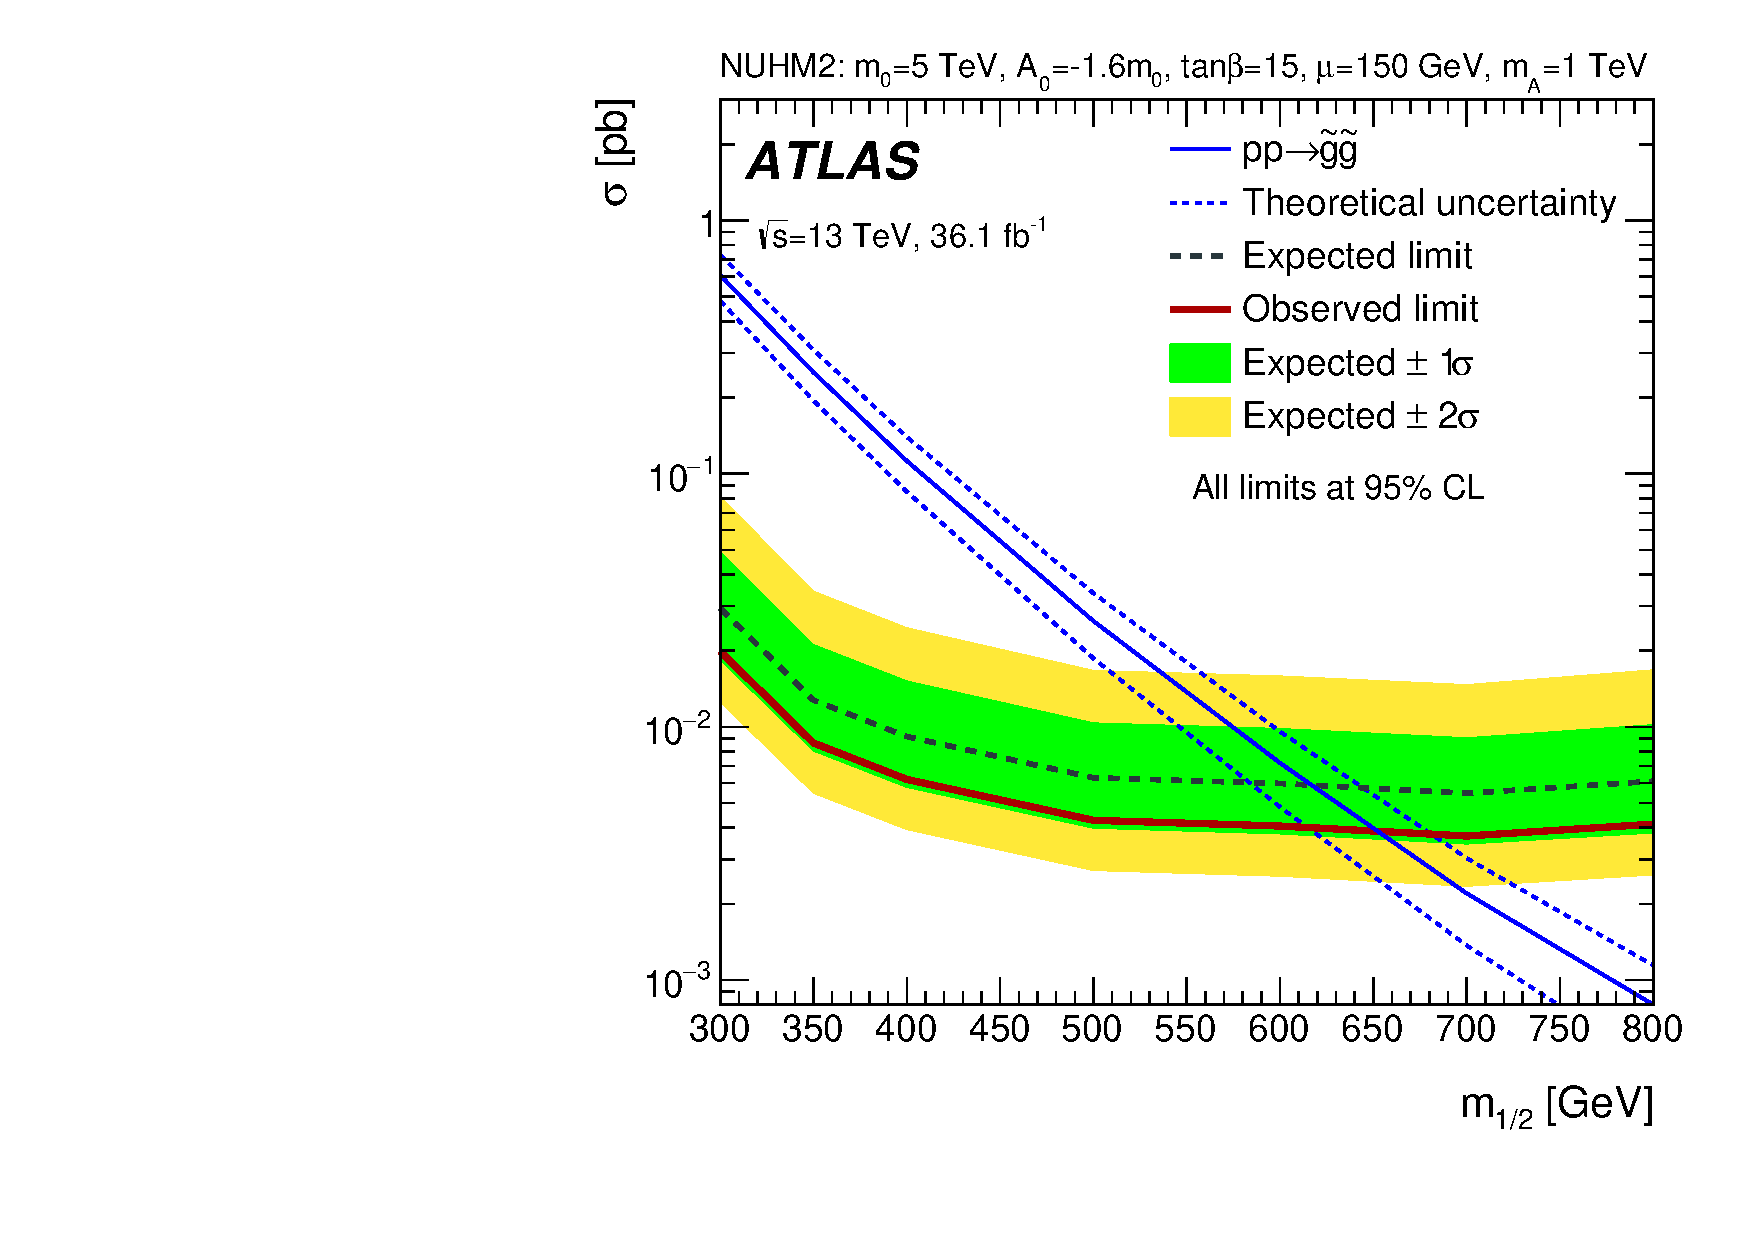
\includegraphics[scale=0.34]{UL_NUHM2.pdf}
    \end{center}
    \caption{The upper limit of the cross-section as a function of $m_{1/2}$ in the NUHM2 model.
    The green and yellow bands around the expected limit are the $\pm 1 \sigma$ and $\pm 2 \sigma$ variations, respectively.}
    \label{tab:app_ss3l_nuhm2_exclusion_plot}
\end{figure}
